\chapter{Datasets}

This chapter describes the datasets used to perform the experiments in this
dissertation.

\section{Related Work}
Many public datasets for evaluating gesture recognition contain only one form
of gesture \cite{marcel99, Ruffieux2013, song11-tracking}. One dataset that
contains different types of gestures is the Chalearn Gesture Dataset (CGD 2011)
\cite{guyon13} which has nine gesture categories corresponding to various
settings and application domains.
 It contains both static postures and dynamic gestures. In this dataset, a static
posture is one in which a single posture is held at the same position for a
certain duration. In this case, the static postures also have
distinct paths so they could be handled by the same method as the dynamic
gestures.
This dataset does not contain gestures with distinct hand poses but arbitrary movement
(Table~\ref{tab:taxonomy} row 2).

\section{YANG Dataset}
Previous related work do not appear to have gesture datasets
that include both gestures with distinct paths and gestures with distinct hand
poses. To evaluate our method, I collected a new dataset named YANG (dichotomY
of in-Air Natural Gestures) which has a vocabulary of 7
one-hand/arm gestures including both path and posture gestures. They
are chosen for possible use in gesture controlled presentation and also to
span over different potential difficulties (see the comments in Table~\ref{tab:gestures}).
Figure shows an example of each
gesture.

\begin{table}[tbh]
\centering
\begin{tabular}{|c|l|l|l|}
\hline
\thead{\#} & \thead{Name of gesture} & \thead{Form} & \thead{Comment} \\
\hline
1 & Swipe left & distinct path & simple path \\
\hline
2 & Swipe right & distinct path & simple path \\
\hline
3 & Circle & distinct path & complex path \\
\hline
4 & Horizontal wave & distinct path & has arbitrary repetitions \\
\hline
5 & Point & distinct hand pose & arbitrary path \\
\hline
6 & Palm forward & distinct hand pose & arbitrary path \\
\hline
7 & Grab & distinct hand pose & arbitrary path \\
\hline
\end{tabular}
\caption{YANG dataset gesture vocabulary.}
\label{tab:gestures}
\end{table}

\begin{figure}[tbh]
\centering
\subfigure[Path gestures]{
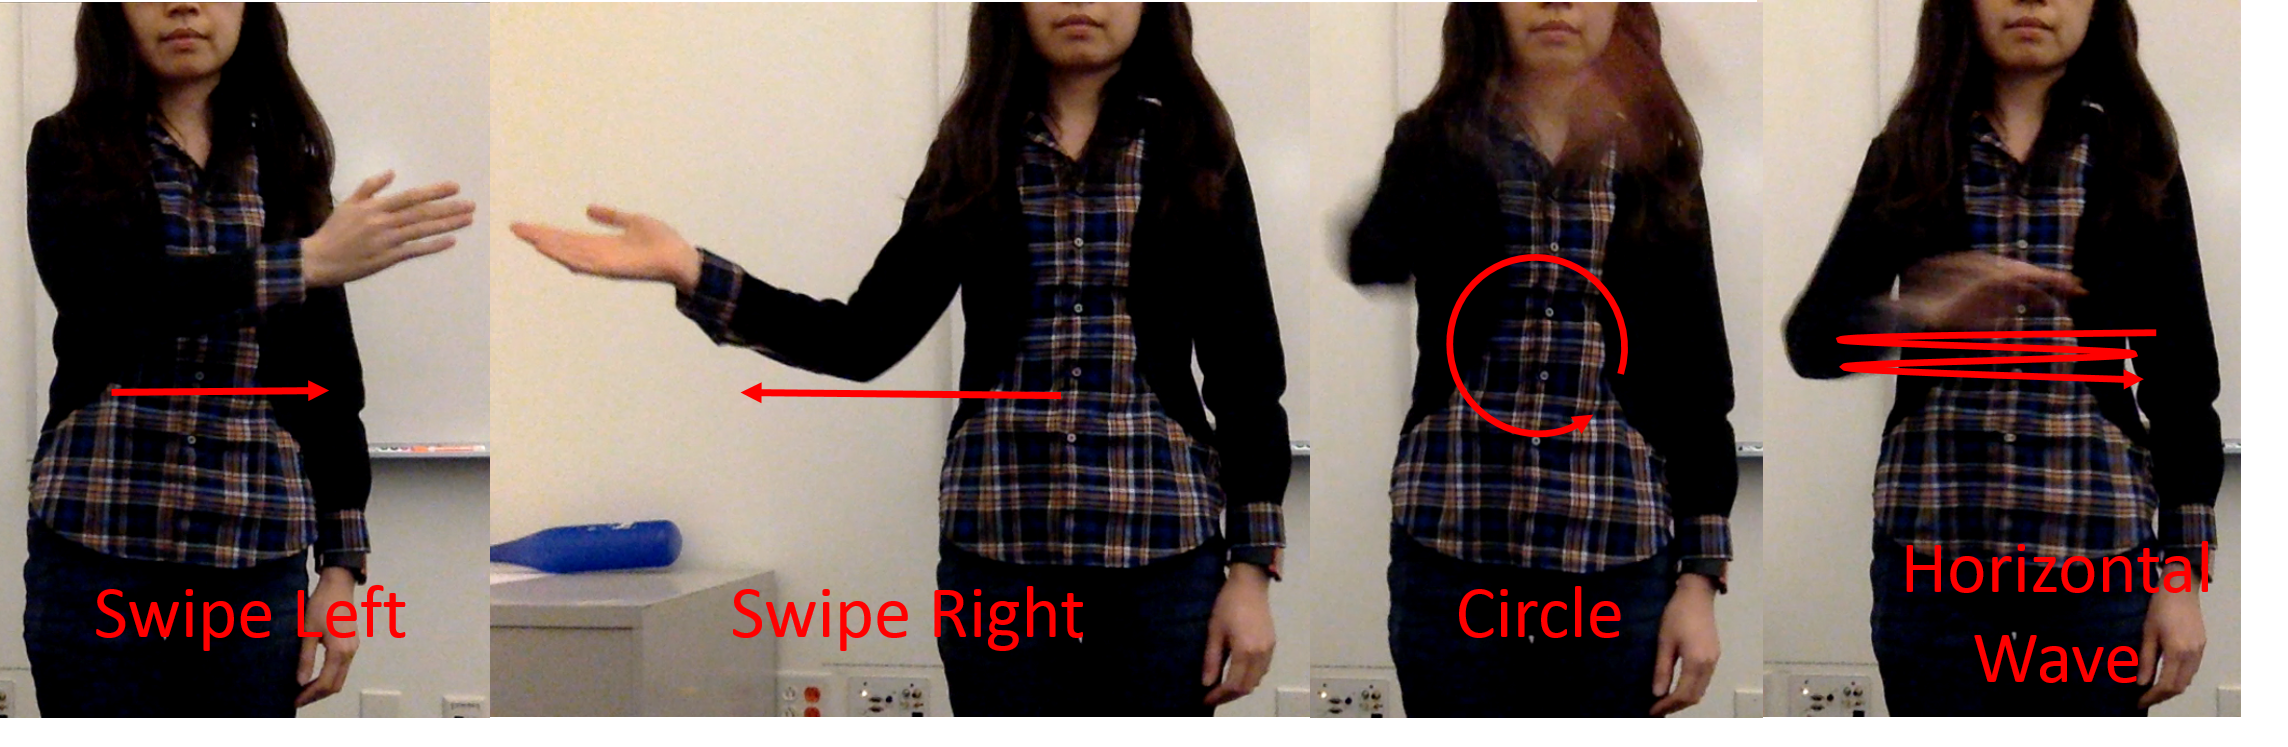
\includegraphics[width=\textwidth]{figures/gestures1.png}
}
\subfigure[Pose gestures with arbitrary movement]{
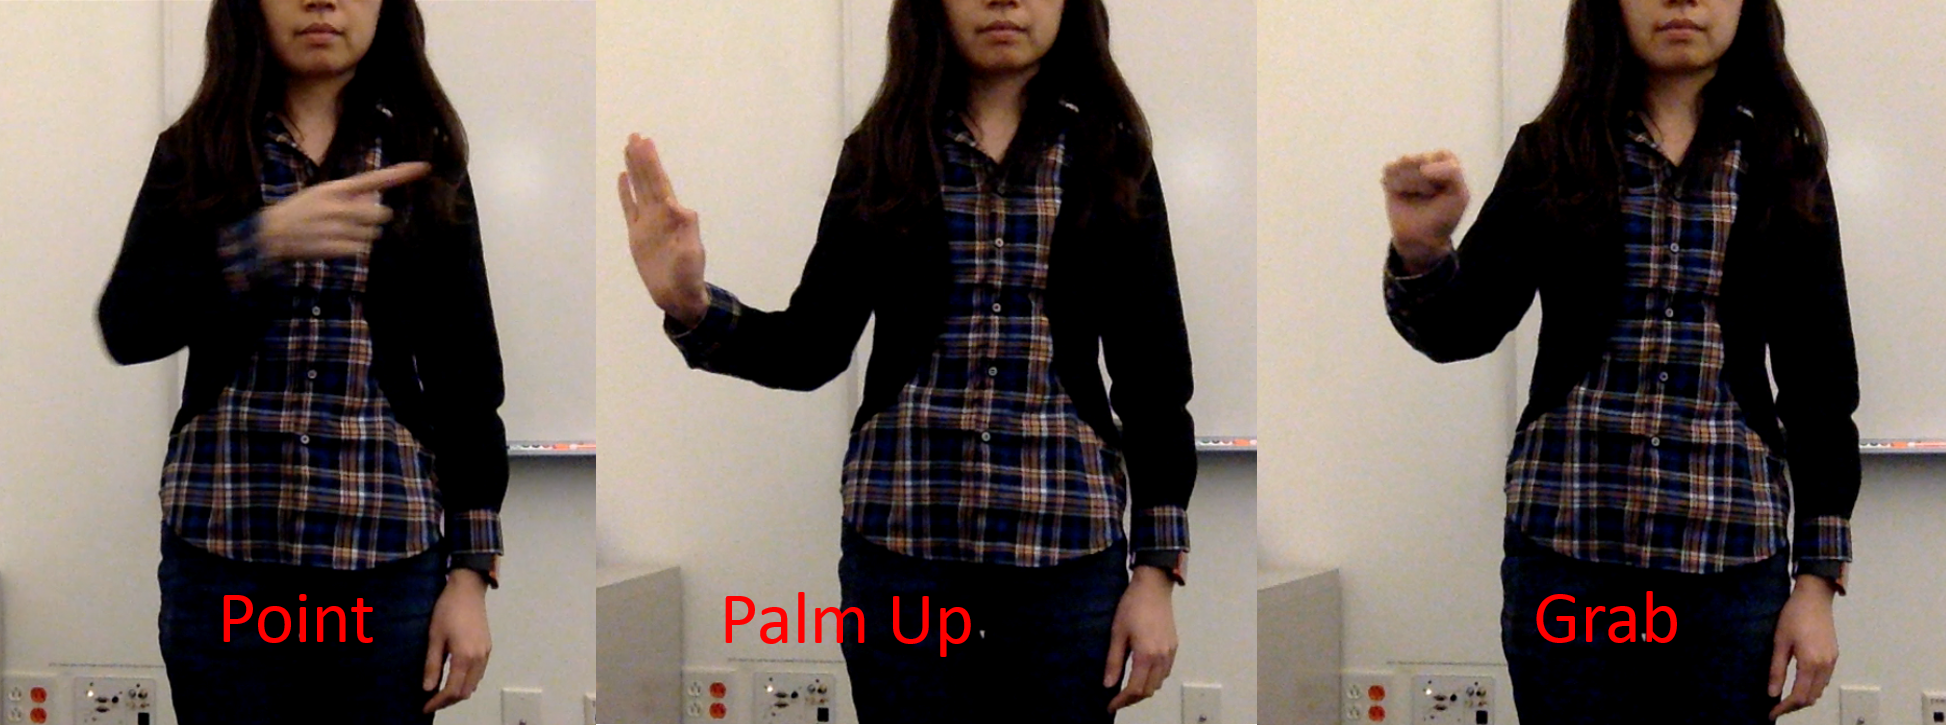
\includegraphics[width=0.75\textwidth]{figures/gestures2.png}
}
\caption{YANG dataset gesture vocabulary.}
\label{fig:yang}
\end{figure}

This dataset presents various features of interest. Table~\ref{tab:challenges} lists
both the challenging and easy aspects of the dataset.

\begin{table}[tbh]
\centering
\begin{tabular}{|l|}
\hline
\thead{Challenging}\\
\hline
\textit{Within each sequence:}\\
Different forms of gestures: path and pose gestures \\
Pose gestures have arbitrary movement \\
Resolution for hands is low \\
Continuous gestures with or without a resting pose \\
Many gesture instances are present \\
Non-gestures may be present \\
\textit{Between sequences:} \\
High variabilities across participants \\
Variations in clothing, skin color, lighting \\
\hline
\thead{Easy} \\
\hline
Fixed camera \\
Near frontal view acquisition \\
Within a sequence the same user \\
Gestures performed by arms and hands \\
Camera framing full body \\
Several data sources: skeletal model, user mask, depth, and RGB \\
Several instances of each gesture for training \\
Single person present in the visual field \\
One hand/arm gestures \\
\hline
\end{tabular}
\caption{Challenging and easy aspects of the dataset.}
\label{tab:challenges}
\end{table}

\subsection{Recording Setup and Procedure}
The dataset contains data from 10 participants each
performing the gestures in 4 sessions. All the participants are university
students.
The participants were shown a video
demonstration of
each gesture\footnote{Video
demonstration of the
gestures: \url{https://www.youtube.com/watch?v=VDDX0TkenTY}} at the beginning.
In each session, the participant stands at about 1.5m from the Kinect
for Windows sensor (version one), and performs each gesture 3 times
according to the text prompts on a screen indicating the name of the gesture to
perform.
The order of the gestures is random and the time between each gesture is random
(between 2s and 6s). The first 2 sessions have ``Rest'' prompts between each
gesture, telling participants to go to the rest position (hands relaxing at the
side of the body), and the second 2 sessions do not have ``Rest'' prompts so
participants can choose to rest or not between consecutive gestures. This too
distinguishes the dataset from previous ones \cite{Ruffieux2013, guyon13} where
gestures are always delimited by rest positions.

Unlike Ruffieux et al. \cite{Ruffieux2013}, we do not show video demonstration
every time the participants perform a gesture because we want a
realistic scenario. In real practice, it is unlikely that a user will follow a
video demonstration every time he/she does a gesture. The result of this is that
there will be more variations among the gestures.

To motivate movement for gestures with distinct hand poses that
require a continuous response, the text prompt asks participants to draw
random letters in the air with the specified hand pose. 

The full corpus contains $
10P \times 4S \times 7G \times 3R = 840$ gesture occurrences
where P = participants, S = sessions, G = unique gestures, R = repetitions per
gesture. There are approximately 96 minutes of continuous recording.

\subsection{Data Formats}

\begin{figure}[tbh]
\centering
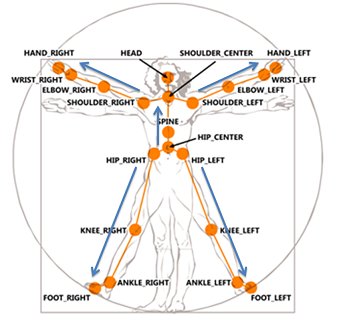
\includegraphics[width=0.7\textwidth]{figures/skeleton.png}
\caption{Skeleton joint positions.}
\label{fig:skeleton}
\end{figure}

The data from the Kinect sensor is recorded in a raw binary format at 30
frame per second (FPS). It includes RGB, depth and skeleton data. Both the RGB
and the depth data have a resolution of $640\times480$px. The skeleton data
contains joint positions for 20 joint types. Figure~\ref{fig:skeleton}\footnote{Image from
\url{http://msdn.microsoft.com/en-us/library/jj131025.aspx} } visualizes these
joint types

During the recording process, the name and the start time (for pre-stroke) for
each gesture are recorded according to the prompts. Due the human reaction time,
the prompt time may not exactly be the true start time of the pre-stroke. I wrote a program to improve the
start pre-stroke and stop post-stroke time labeling based on the initial
recorded timings by automatically detecting the rest positions. There is no
ground truth time labels for start and stop of nucleus phases.

\subsection{Qualitative Observations}
We find that there is considerable variations in the way participants perform
each gesture even they were given the same demonstration video. Major variations
are observed in speed, the magnitude of motion, the paths and hand poses.

For example, some participants do the swipe left and right gestures in a rather
straight horizontal line, while others have a more curved path.  Some
participants do swipe left and right with a palm forward pose while others have
less distinct hand poses (hand is more relaxed). Some participants start
the circle gesture at the bottom, while others start at the top. Some
participants do the ``circle'' gesture in clockwise direction while others do it
in anti-clockwise direction. Figure~\ref{fig:compare-swipe-right} shows
an illustration of such differences. However, within each participant, the
intra-class variation of gestures is smaller, although still present.

\begin{figure}[tbh]
\centering
\includegraphics[width=\textwidth]{figures/compare_swipe_right.png}
\caption{Differences between participants for the same swipe right gesture. 
The first row shows that a user does the swipe right gesture in a straight
horizontal path with a palm forward pose; the second row shows that another user
does the same gesture in a curve path with less distinct poses.}
\label{fig:compare-swipe-right}
\end{figure}

\subsection{User Preferences}\label{sec:preferences}
We did a survey with the participants on questions that can influence
gesture interface design. Below are the aggregated results:
\begin{itemize}
  \item User differences: As an example to show user differences, we asked
  the participants how they would prefer to do the ``circle'' gesture. 54\%
  of them prefer doing the ``circle'' gesture in clockwise direction, 15\% in
  anti-clockwise direction, and 31\% do not care.
  \item Predefined gestures versus user defined gestures: 90\%
  of the participants prefer to be able to define their own gestures if necessary while 10\% of them prefer to follow prefined
  gestures completely. No one prefers to use a system without any predefined
  gestures either.
  \item How to define gestures: 80\% prefer defining gesture by 
  performing the gestures themselves; no one prefers to
  define gestures solely via rules written in terms of positions and directions
  of movement of the hands.
  However 20\% prefer to be able to do both.
  \item Number of repetitions per gesture for training: 50\% are willing to give a
  maximum of 4 -- 6 examples, 40\% are willing ot give 1 -- 3 examples, and 10\%
  are willing to give more than 13 examples. So the average maximum is about 5
  repetitions.
  \item Number of gestures for an application: 80\% think 6--10 gestures are
  appropriate and easy to remember for a given application, while 20\% prefers 1
  -- 5 gestures, giving an average of 7 gestures.
  \item Intuitiveness of the gesture vocabulary for PowerPoint presentation:
  the average score is 4 out of 5 where 5 is very intuitive.
\end{itemize}

\subsection{Implications for Gesture Interaction Interface}
Based on our observation of the large variation in gesture execution among
users and small variations within users, and the fact that a majority of
participants preferring defining their own gestures if they do not like the
predefined gestures, I suggest that it may be more important to optimize user
dependent recognition and user adaptation. As no one prefers to define their own
gesture at the very beginning, it also means that having a reasonable predefined gesture set and
basic user independent model for recognition will be useful too.

Recognition methods based on examples will allow users to train models of their
own gestures easily. We also need to develop methods that
require relatively few training examples and fast training speed.

\section{ChAirGest Dataset}
The ChAirGest dataset~\cite{Ruffieux2013} is a publicly available
dataset\footnote{\url{https://project.eia-fr.ch/chairgest/Pages/Download.aspx}}
for the ongoing open challenge on Multimodal Mid-Air Gesture Recognition for
Close
HCI\footnote{\url{https://project.eia-fr.ch/chairgest/Pages/Scoreboard.aspx}}.
Although the dataset only has path gestures, it has other interesting features
which are relevant for evaluating the methods in this thesis:
\begin{itemize}
  \item It has data from both a Kinect sensor and IMU sensors, allowing me to
  evaluate the generalizability of my methods for different sensor input and
  compare recognition performance for different combinations of sensor input. 
  \item It has ground truth labeling of
  pre-stroke, nucleus and post-stroke phases. Few datasets have gesture phase
  labeling. This dataset allows me to evaluate my gesture phase segmentation method.
  \item It represents the scenario where a person sits in front of a
  desk working on a computer. Because of the absence of the full body and the
  presence of the distracting foreground (the desk), the Kinect skeleton
  tracking is less robust. This allows me to evaluate my salience based hand
  tracking method in the case where the skeleton tracking fails.
  \item It contains three different rest poses selected according to common user
  positions when sitting in front of a computer: ``hands on the table'' when
  working/typing, ``elbows on the table, hands joined under chin'' when thinking
  and ``hands on the belly'' when watching a movie. These variations, which
  closely mimic the reality, present challenges to hand tracking, as well as to
  detecting the gesture phases as the pre-stroke and the post-stroke are
  affected the rest positions.
\end{itemize}

\subsection{Gestures}
The dataset contains a vocabulary of 10 one-hand/arm gestures focusing on close
HCI (Table~\ref{tab:chairgest-vocab}). The vocabulary has been chosen to span
over different potential difficulties which include variations in paths, hand rotations, and hand poses.
Some gestures have overlapping paths but different hand poses. This is
to promote algorithms using fusion from multiple sensors.

\begin{table}[tbh]
\centering
\begin{tabular}{|l|l|}
\hline
\thead{\#} & \thead{Name of gesture} \\
\hline
1 & Shake hand \\
\hline
2 & Wave hello \\
\hline
3 & Swipe right \\
\hline
4 & Swipe left \\
\hline
5 & Circle palm rotation \\
\hline
6 & Circle palm down \\
\hline
7 & Take from screen \\
\hline
8 & Push to screen \\
\hline
9 & Palm-down rotation \\
\hline
10 & Palm-up rotation \\
\hline
\end{tabular}
\caption{ChAirGest gesture vocabulary.}
\label{tab:chairgest-vocab}
\end{table}

The dataset contains 10 participants, each doing 4 recording sessions with 2
different lighting conditions (dark and normal). In a recording session, the
participant performs once each gesture class for each resting posture. The full
corpus contains $10P\times (2L \times [2S \times 10G \times 3R]) = 1200$
gesture occurrences, where $S$ = subject, $L$ = lighting condition, $S$ =
session, $G$ = unique gesture, and $R$ = resting posture.

\subsection{Recording Setup}
The participant sits on a chair in front of a desk as if working on a computer.
He/she wears 4 Xsens IMUs attached under his/her clothes on his/her shoulder, arm, wrist and hand.
A Kinect for Windows records the scene from the top of a computer screen with a
30\textdegree downward angle.

\subsection{Data Formats}
The Kinect binary format contains the RGB and the depth streams along with the
3D skeleton representation at 30Hz acquired using the official SDK. Each Xsens IMU
provides information in: linear acceleration, angular acceleration,
magnetometer, Euler orientation and orientation quaternion at 50Hz.

\subsection{Performance Metric}\label{sec:chairgest-metric}
The challenge uses a combination of existing event-based metrics and a novel
time-based metric to evaluate performance. The two event-based metrics are
precision and recall which are combined to compute an $F_1$ score. Let
$t_{gt\_start\_nucleus}$ and $t_{gt\_stop\_nucleus}$ be the ground truth start time and stop time of a gesture nucleus respectively,
and let $t_{alg\_start\_nucleus}$ and $t_{alg\_stop\_nucleus}$ be the
corresponding timings returned by a recognition algorithm for the same gesture.
A detected gesture event is correct if only if the label of the gesture is
correct and the timings satisfy the following condition
\begin{align*}
|t_{gt\_start\_nucleus} - t_{alg\_start\_nucleus}| &< 0.5\times
(t_{gt\_stop\_nucleus} - t_{gt\_start\_nucleus}) \quad \text{\&\&} \\
|t_{gt\_stop\_nucleus} - t_{alg\_stop\_nucleus}| &< 0.5\times
(t_{gt\_stop\_nucleus} - t_{gt\_start\_nucleus})
\end{align*}
Figure~\ref{fig:true-positive} shows an example comparing the results from two
algorithms. Even though both of them have correct labels for the detected
gesture nucleus, the result from Algorithm 1 is not considered correct because
the time discrepancy is larger than the allowed tolerance which is half of the
ground truth duration of the gesture nucleus.

\begin{figure}[tbh]
\centering
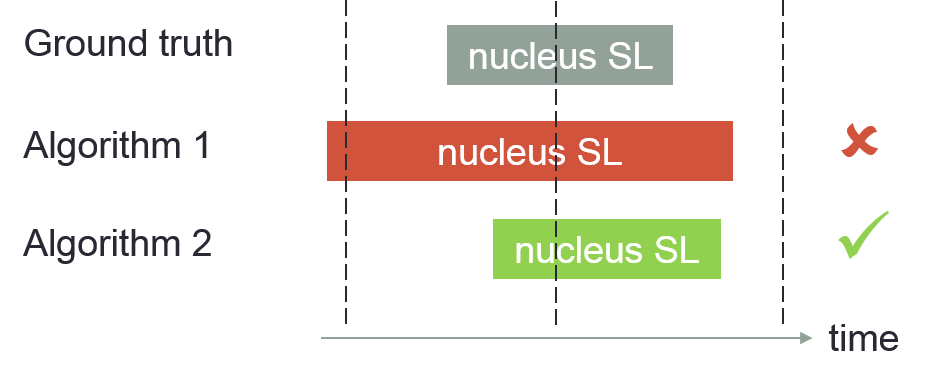
\includegraphics[width=0.7\textwidth]{figures/true_positive.png}
\caption{Even though the gesture nucleus label detected by Algorithm 1 is
correct (SL stands for ``swipe left''), the start time difference from the
ground truth is too large (larger than half of the ground truth nucleus
duration), and hence, it is not considered as a correct detection. The detection
from Algorithm 2 is considered correct.}
\label{fig:true-positive}
\end{figure}

The time-based metric is used to measure the gesture spotting performance and
the accuracy of temporal segmentation. The metric is named \textit{Accurate
Temporal Segmentation Rate} (ATSR) and represents a measure of the performance
in terms of accurately detecting the start and stop timings of all correctly
detected gesture nuclei. The ATSR is computed as follows: for each correctly detected gesture
occurrence, the \textit{Absolute Temporal Segmentation Error} (ATSE) is computed
according to Equation~\ref{eqn:atse}; the ATSR metric is computed for a
particular sequence with $n$ correctly detected gestures according to
Equation~\ref{eqn:atsr}.
\begin{align}
ATSE &= \frac{|t_{gt\_start\_nucleus} - t_{alg\_start\_nucleus}| +
|t_{gt\_stop\_nucleus} - t_{alg\_stop\_nucleus}|}{t_{gt\_stop\_nucleus} -
t_{gt\_start\_nucleus}} \label{eqn:atse} \\
ATSR &= 1 - \frac{1}{n}\sum_{i=1}^nATSE(i)
\label{eqn:atsr}
\end{align}

The final single metric is evaluated using a combination of $F_1$ score and ATSR
according to Equation~\ref{eqn:perf}. The $F_1$ score has twice more importance
than the ATSR as correct recognition of gestures remains more important.
\begin{align}
Perf = 5\times \frac{ATSR\times F_1}{4\times ATSR + F_1}\label{eqn:perf}
\end{align}
